\section{Analisi dei requisiti}
\subsection*{Individuazione dei requisiti}
La prima attività svolta durante lo \textit{stage}, nella prima settimana è stata conosce le persone coninvolte nel progetto e
discutere con loro gli obiettivi e le aspettative del progetto.\\
Successivamente, ho iniziato a studiare i nuvi linguaggi di programmazione e tecnologie che avrei utilizzato durante lo svolgimento delle attività.\\
La seconda settimana invece, ho effettuato l'analisi dei requisiti, attività cruciale condotta 
insieme ai membri del \textit{team}. Con questo processo ho potuto identificarei requisiti 
funzionali, di vincolo e definire i casi d'uso del sistema.

Adottando un approccio in linea con la metodologia agile, ho optato per una raccolta requisiti di tipo incrementale. 
Questo metodo ha permesso una maggiore flessibilità, consentendo aggiornamenti e modifiche dei requisiti in base alle 
mutevoli esigenze del \textit{team} e dell'evoluzione del progetto.

Il primo passo è stato la creazione di un nuovo documento su Confluence. Ho iniziato inserendo le informazioni 
generali del progetto, quali il nome, il \textit{team} coinvolto e una descrizione sintetica. Successivamente, 
ho definito e documentato le convenzioni adottate per la stesura del documento, come la nomenclatura specifica per 
i requisiti e i casi d'uso.

Nella fase successiva, ho proceduto con la stesura effettiva dei requisiti. Inizialmente, ho optato per una 
suddivisione basata sul tipo di requisito, differenziando tra funzionali e di vincolo attraverso due tabelle distinte. 
Tuttavia, nel corso dell'analisi, abbiamo introdotto un ulteriore livello di suddivisione. Questo ci ha permesso di 
classificare i requisiti anche in base al componente del sistema a cui si riferiscono, ovvero \textit{backend}, 
\textit{frontend} e \textit{plugin} Gradle.

Conforme alle aspettative e alla natura agile del progetto, i requisiti sono stati soggetti a continui aggiornamenti 
e modifiche nel corso dello sviluppo. Un esempio significativo è stato l'inserimento dei requisiti facoltativi, 
che inizialmente non erano stati presi in considerazione, ma che si sono rivelati fondamentali per rispondere in 
modo più completo alle esigenze del progetto.

\begin{figure}[!h] 
  \centering 
  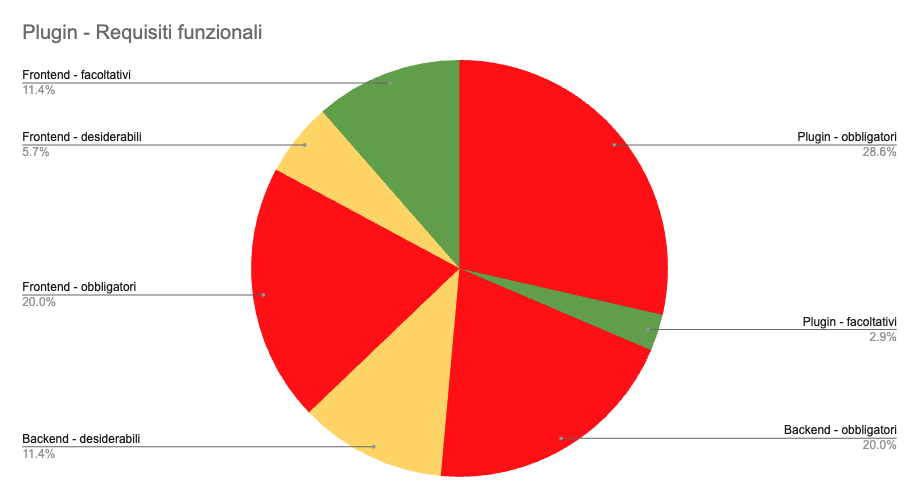
\includegraphics[width=1\columnwidth]{pie-req} 
  \caption{Grafico a torta che mostra la suddivisione in percentuale dei vari requisiti.}
  \label{fig:pie-req}
\end{figure}
\noindent Nella figura \ref*{fig:pie-req} è possibile vedere la suddivisione in percentuale dei requisiti, 
suddivisi come descritto in precedenza.\\
Nella figura \ref*{fig:req-per-importanza} è possibile vedere la suddivisione dei requisiti in base all'importanza.
\begin{figure}[!h] 
  \centering 
  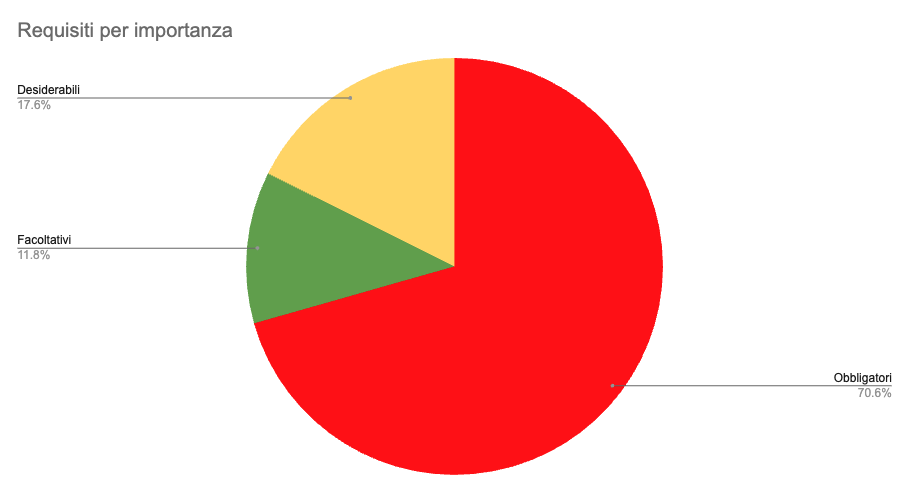
\includegraphics[width=1\columnwidth]{req-per-importanza} 
  \caption{Grafico a torta che mostra la suddivisione dei requisiti in base all'importanza.}
  \label{fig:req-per-importanza}
\end{figure}

\subsection{Tracciamento dei requisiti}
Ad ogni requisito scritto in Confluence ho associato un codice univoco, che mi ha permesso di tracciarlo.
Il codice che ho utilizzato per identificarli è il seguente:
\begin{align*}
  \textbf{R[F/V]-[O/D]-[B/F/P]-[001]}
\end{align*}
Nello specifico:
\begin{itemize}
    \item \textbf{RF}: requisito funzionale, \textbf{RV}: requisito di vincolo;
    \item \textbf{O}: obbligatorio, \textbf{D}: desiderabile, \textbf{F}: facoltativo;
    \item \textbf{P}: componente del sistema a cui si riferisce, \textbf{B}: \textit{backend}, \textbf{F}: \textit{frontend}, \textbf{P}: \textit{plugin} Gradle;
    \item \textbf{001}: numero progressivo del requisito.
\end{itemize}

\noindent Per il tracciamento dei requisiti, ho utilizzato un metodo efficace utilizzando Confluence e Jira. 
Nella tabella dei requisiti, che ho creato su Confluence e identificabile tramite la figura \ref*{fig:jira-confluence-requisiti}, 
ho inserito una nuova colonna. In questa colonna, ho inserito il riferimento alla \textit{issue} di 
Jira corrispondente a ciascun requisito.\\
Questa integrazione tra Confluence e Jira ha permesso di collegare direttamente ogni requisito a una specifica 
\textit{issue} di Jira, che ne dettaglia l'implementazione. Grazie a questo collegamento, ho ottenuto una visione più 
completa e dettagliata del progetto, migliorando notevolmente la precisione nel tracciamento dei requisiti.\\
Inoltre, ho sfruttato la funzionalità di visualizzazione automatica in modalità \textit{read-only} su Confluence. 
Questo ha permesso di consultare direttamente nella tabella dei requisiti le informazioni essenziali relative alle \textit{issues} 
di Jira, come lo stato di avanzamento e le descrizioni dettagliate, quando necessario.

Ogni \textit{issue} l'ho collegata ad un'epica, che rappresenta un insieme di \textit{issues} correlate tra loro. In tutto ho creato 4 epiche,
una per ogni componente del progetto (\textit{backend}, \textit{frontend}, \textit{plugin} Gradle e analisi).\\
\begin{figure}[!h] 
  \centering 
  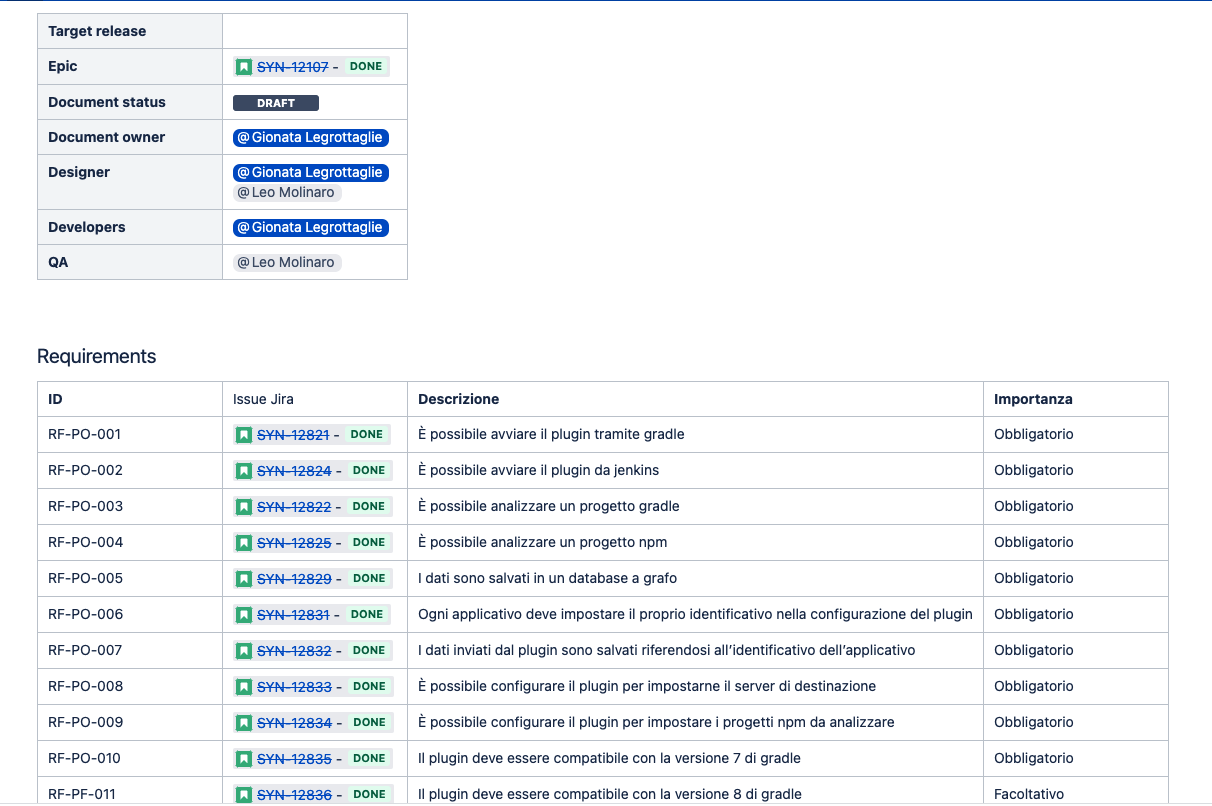
\includegraphics[width=.9\columnwidth]{jira-confluence-requisiti} 
  \caption{Tabella che mostra il tracciamento dei requisiti su Confluence, con il collegamento a Jira.}
  \label{fig:jira-confluence-requisiti}
\end{figure}

Tramite Jira ho creato un \textit{board} per il progetto, che mi ha permesso di visualizzare in modo chiaro e 
semplice lo stato di avanzamento del progetto, vedi la figura \ref*{fig:board-jira}.
All'interno di questa \textit{board} è possibile visualizzare, per ogni \textit{record} della tabella, il tipo di \textit{issue}, il vodice, la priorità, lo stato,
la persona assegnata, la stima in giorni/ore e, per l'intero \textit{sprint}, la stima totale in giorni/ore.\\


\begin{figure}[!h] 
  \centering 
  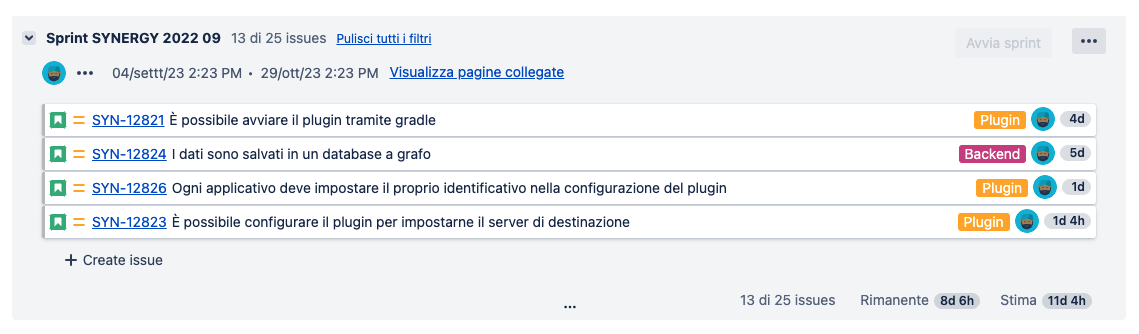
\includegraphics[width=1\columnwidth]{board-jira} 
  \caption{\textit{Board} di Jira che mostra lo stato di avanzamento del progetto.}
  \label{fig:board-jira}
\end{figure}

\noindent Jira offre una gamma di funzionalità avanzate, tra cui spicca la capacità di creare dei \textit{plan}. 
Questa funzionalità si rivela particolarmente utile nella pianificazione delle \textit{issues}, consentendo di organizzarle 
efficacemente in base alle loro date di inizio e fine, permettendoti di avere una visualizzazione grafica del 
progetto attraverso un grafico di \textit{gantt}. \\ Questo grafico rappresenta visivamente le \textit{issues} 
in relazione alle loro date di inizio e fine, offrendo una panoramica chiara e immediata dello stato di avanzamento del progetto, mettendo
in risalto anche le \textit{milestone} prefissate nel piano di lavoro.\\ 
Inoltre, una funzionalità di Jira permette di modificare e riallocare le \textit{issues} con facilità, 
adattandosi dinamicamente alle esigenze del progetto in corso.
